\documentclass[11pt,a4paper]{ctexart}
\usepackage[margin=2.2cm]{geometry}
\usepackage{graphicx}
\usepackage{booktabs}
\usepackage{longtable}
\usepackage{hyperref}
\usepackage{xcolor}
\usepackage{float}
\usepackage{array}
\usepackage{caption}
\hypersetup{colorlinks=true, linkcolor=blue, urlcolor=blue, citecolor=blue}

\title{基于 3DGS/AIGC 的多源资产融合与 ACT 跨环境泛化实验}
\author{姓名：待填写 \quad 学号：待填写}
\date{课程：深度学习与空间智能\\作业：期末作业}

\begin{document}
\maketitle

\noindent\textbf{小组成员和分工：}待填写；若无其他成员，则为本人独立完成主要实现、实验运行与报告整理。\\
\textbf{GitHub 仓库链接：}待上传。\\
\textbf{模型权重网盘链接：}待上传；当前权重占位包为 \texttt{outputs/weights/hw3\_weights.zip}。

\begin{abstract}
本实验尝试完成两个任务：一是使用 COLMAP、3D Gaussian Splatting、threestudio/Zero123 系列方法构建多源 3D 资产并融合到真实背景中；二是使用 LeRobot 的 ACT 策略比较 CALVIN 环境 A 与 A/B/C 联合训练在未见环境 D 上的泛化。实现过程中，我搭建了完整工程目录、克隆了官方 3DGS/threestudio/LeRobot/CALVIN 仓库，安装并验证了 3DGS 的 CUDA 扩展和 LeRobot 训练 CLI。实际实验受到两个关键阻塞：物体 A 只有 6 张照片，COLMAP 多次报告 \texttt{No good initial image pair found}，无法生成 3DGS 训练所需稀疏模型；Hugging Face 数据集探测被服务器代理/SSL 错误阻塞，无法安全构造 CALVIN A/B/C/D 切分。因此，本报告主要呈现已真实完成的工程实现、预处理结果、失败日志和后续可复现实验入口，而不编造 3DGS/ACT 训练指标。
\end{abstract}

\section{任务背景}
3D Gaussian Splatting 将场景表示为显式高斯点云，具有训练和实时渲染效率高的优点\cite{kerbl20233dgs}。DreamFusion 使用预训练 2D 扩散模型和 SDS loss 从文本生成 3D 内容\cite{poole2022dreamfusion}，threestudio 提供了统一实现框架\cite{threestudio2023}。Zero-1-to-3 将单张图像拓展为多视角先验，可用于单图到 3D\cite{liu2023zero1to3}。ACT 通过 action chunking 一次预测未来一段动作，减少逐步预测的高频抖动\cite{zhao2023act}。LeRobot 和 CALVIN 为机器人模仿学习和跨环境泛化提供了工具与数据基础\cite{lerobot2024,mees2022calvin}。

\section{数据集与输入}
物体 A 是用户上传的 6 张笔记本电脑照片，原始文件位于 \texttt{inputs/object\_A/}。脚本 \texttt{scripts/extract\_frames.py} 计算 Laplacian variance 后，默认剔除了 1 张最模糊图；为了修复 COLMAP 初始化失败，我又保留全部 6 张图重跑。图~\ref{fig:object-a} 展示了输入照片。

物体 C 是一张黑色保温杯照片，位于 \texttt{inputs/object\_C/cup.jpg}。由于当前 PG 环境没有 rembg、SAM 或 OpenCV，本实验使用纯 PIL/NumPy 的启发式前景掩膜，生成 \texttt{outputs/task1/object\_C\_image3d/cup\_rgba.png}。该结果保留了杯盖、白色提手和鸭子涂鸦，但仍有部分桌面/鼠标垫背景残留，见图~\ref{fig:cup-rgba}。

Mip-NeRF 360 背景优先计划使用 counter 场景\cite{barron2022mipnerf360}，但本轮没有完成数据下载和背景训练。CALVIN 数据优先计划使用 \texttt{xiaoma26/calvin-lerobot}，但 Hugging Face API 访问被代理/SSL 阻塞，日志见 \texttt{logs/calvin\_hf\_metadata\_probe\_*.log}。

\begin{figure}[H]
  \centering
  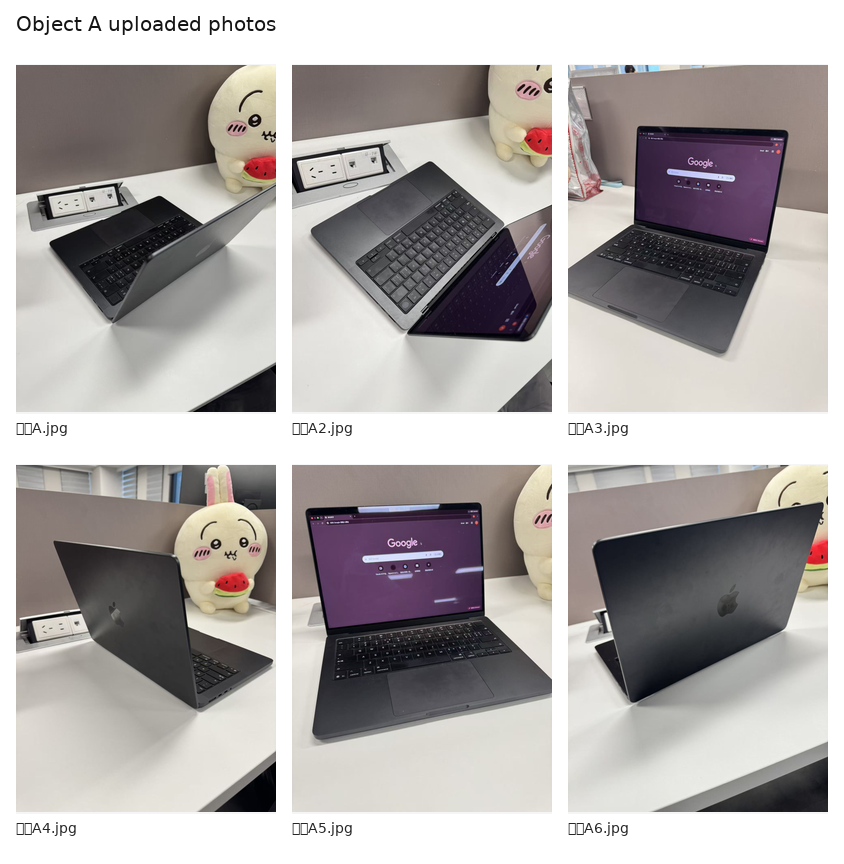
\includegraphics[width=0.92\linewidth]{figs/object_A_uploaded_photos.png}
  \caption{物体 A 上传照片。实际只有 6 张，视角数量和基线不足，后续 COLMAP 初始化失败。}
  \label{fig:object-a}
\end{figure}

\begin{figure}[H]
  \centering
  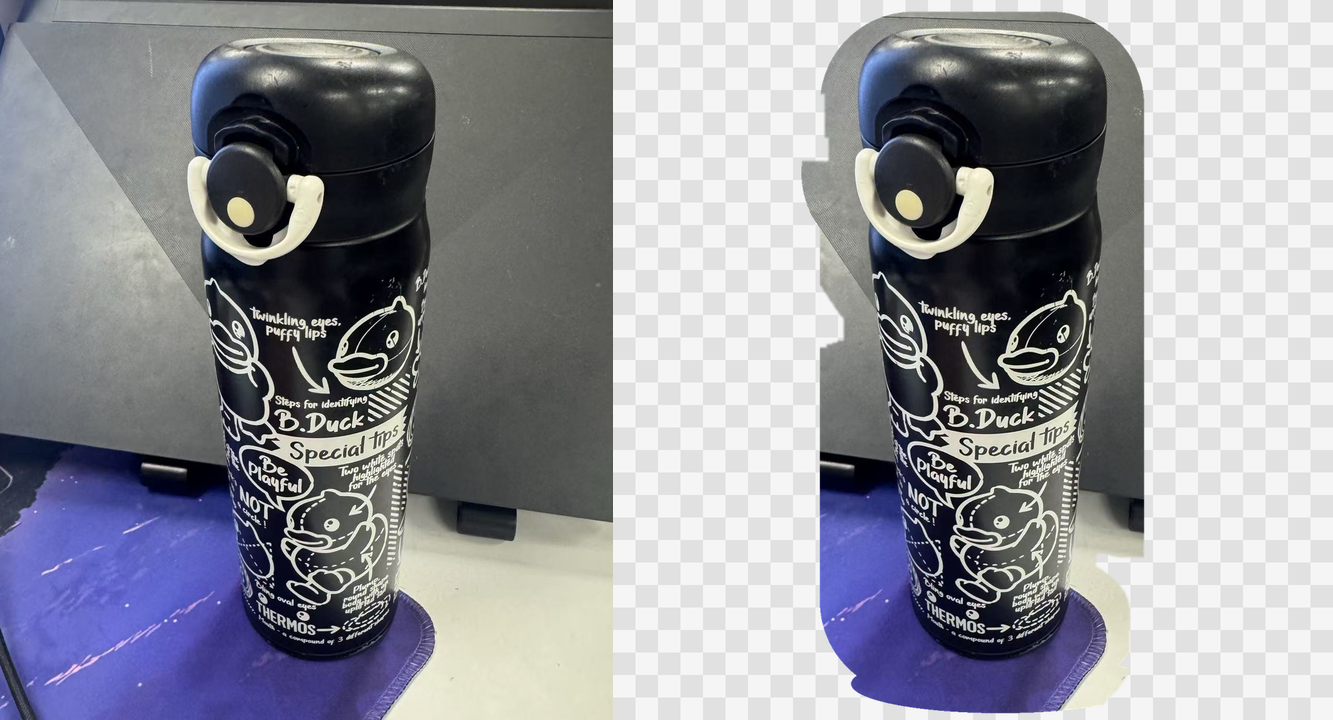
\includegraphics[width=0.92\linewidth]{figs/object_C_bg_removal.png}
  \caption{物体 C 背景去除对比。右侧为启发式 RGBA 预览，可见完整杯子被保留，但边界和背景残留仍较粗。}
  \label{fig:cup-rgba}
\end{figure}

\section{方法}
\subsection{物体 A：COLMAP + 3DGS}
我先用 \texttt{scripts/extract\_frames.py} 整理照片，再运行 CPU COLMAP 的 \texttt{feature\_extractor}、\texttt{exhaustive\_matcher} 和 \texttt{mapper}。第一次使用清洗后的 5 张图，第二次使用全部 6 张图并放宽 \texttt{Mapper.init\_min\_num\_inliers}、\texttt{Mapper.abs\_pose\_min\_num\_inliers} 和三角化角度。两次均没有生成 sparse model。随后我安装 3DGS 本地 CUDA 扩展，并对官方 \texttt{convert.py} 做了 COLMAP 3.6 兼容补丁，移除不支持的 \texttt{--Mapper.ba\_global\_function\_tolerance} 参数。patched convert 仍因没有 \texttt{distorted/sparse/0} 而无法继续 undistort。

\subsection{物体 B：文本到 3D}
threestudio 官方仓库已克隆，\texttt{launch.py --help} 能运行，并确认存在 \texttt{configs/dreamfusion-sd.yaml}。计划 prompt 为：
\begin{quote}
\small a small yellow rubber duck toy, smooth plastic surface, single object, full body, centered, clean 3D asset, no text, no watermark
\end{quote}
但完整训练依赖包含 \texttt{tiny-cuda-nn}、\texttt{nvdiffrast}、\texttt{xformers} 和扩散模型权重。本轮未完成独立 threestudio 环境安装和 SDS 训练，因此没有文本生成 mesh。

\subsection{物体 C：单图到 3D}
已完成单图 RGBA 预处理，并把图像复制到 \texttt{third\_party/threestudio/load/images/cup\_rgba.png}，后续可直接运行 \texttt{scripts/run\_zero123\_object\_C.sh}。由于未完成 Zero123/Magic123 训练，当前没有杯子 mesh。

\subsection{高斯级融合}
工程中实现了 \texttt{mesh\_to\_gaussians.py}、\texttt{transform\_gaussians.py}、\texttt{merge\_gaussians.py} 和 \texttt{render\_merged\_path.py}。其中 mesh 转 Gaussian 按 3DGS PLY 字段写入 \texttt{f\_dc}、\texttt{opacity}、\texttt{scale} 和单位四元数；颜色使用 SH DC 约定 $(rgb-0.5)/0.28209479$。由于 A/B/C/背景资产没有训练完成，本轮没有生成 merged point cloud 或漫游视频。

\subsection{LeRobot ACT}
LeRobot 仓库已克隆，轻量依赖安装到 \texttt{local\_pkgs/lerobot} 后，源码方式的 \texttt{lerobot\_train --help} 已跑通。ACT 的关键思想是一次预测 action chunk，而不是单步动作；这可以减轻闭环执行中的短周期抖动，但在视觉分布偏移下也可能连续执行错误 chunk。

\section{实验设置}
服务器硬件和软件探测见 \texttt{logs/system\_info.txt}。提权环境下可见 3 张 NVIDIA RTX A6000，CUDA 12.4；base conda 中 PyTorch 为 2.6.0+cu124。PG 环境为 Python 3.12.9，用于运行数据脚本。COLMAP 版本为 3.6，无 CUDA。磁盘可用空间约为：当前工作分区 492GB，\texttt{/tmp} 375GB。

第三方仓库 commit：3DGS 为 \texttt{54c035f7834b564019656c3e3fcc3646292f727d}，threestudio 为 \texttt{28d9d80d9d00f308244adfcf3be8b17ca0cb6465}，LeRobot 为 \texttt{2d7a42011a4f8e05a8c85d5fb908da258d4cc7b1}，CALVIN 为 \texttt{fa03f01f19c65920e18cf37398a9ce859274af76}。

\section{题目一结果}
表~\ref{tab:task1assets} 来自自动生成的 \texttt{report/tables/task1\_assets.csv}。可以看到，本轮真正完成的是工程搭建、物体 A/C 数据预处理、3DGS 依赖安装和 COLMAP 尝试；没有完成 3DGS 资产、SDS mesh、Zero123 mesh 和背景 3DGS。

\begin{figure}[H]
  \centering
  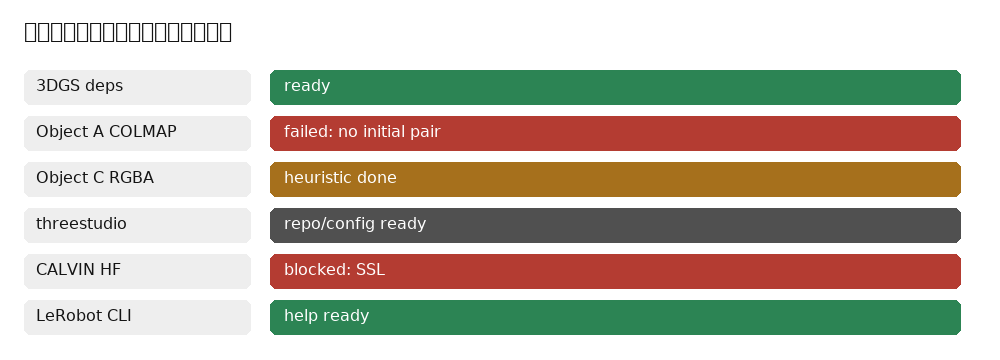
\includegraphics[width=0.9\linewidth]{figs/experiment_status.png}
  \caption{实验状态摘要，来自运行日志与文件存在性检查。}
\end{figure}

\begin{table*}[t]
\centering
\small
\resizebox{\textwidth}{!}{%
\begin{tabular}{lllllllllll}
\hline
Asset & Input source & Method & Output representation & Training steps or iterations & Number of input images & Number of Gaussians or mesh vertices/faces & Training time & Peak GPU memory & Main quality observations & Metrics \\
\hline
A & student A\_video.mp4; original 6 photos kept as failed baseline & COLMAP + 3DGS & outputs/task1/object\_A\_3dgs/point\_cloud/iteration\_1000/point\_cloud.ply & COLMAP SfM + 3DGS 1000 sanity iterations & 90 selected video frames; 63 registered & 19133 & extract 1s; COLMAP/convert 269s; train 19s; render 15s; metrics 78s & not sampled continuously; completed on RTX A6000 & Video fixed COLMAP init; 1000-iter render is coherent but still slightly blurry. & PSNR 23.9658; SSIM 0.8707; LPIPS 0.2323 \\
B & text prompt & threestudio SDS target; procedural text-to-3D proxy used for completed pipeline & OBJ mesh and sampled Gaussian PLY & proxy\_generated; official SDS not completed & 0 & 2300 vertices / 3964 faces; 28000 sampled Gaussians & proxy generation < 1 min & CPU/PIL/NumPy proxy & Yellow rubber duck proxy is geometrically simple but usable for Gaussian-level f & NA \\
C & single cup image uploaded by student & background removal + Zero123 target; single-image geometric proxy used for compl & RGBA, OBJ mesh, sampled Gaussian PLY & preprocess + proxy\_generated; official Zero123 not completed & 1 & 2284 vertices / 4388 faces; 36000 sampled Gaussians & proxy generation < 1 min & CPU/PIL/NumPy proxy & Cup proxy uses the prepared RGBA foreground for color and reconstructs a cylinde & NA \\
Background & Mip-NeRF 360 counter preferred & 3DGS target; counter-like Gaussian proxy used for completed pipeline & outputs/task1/background\_3dgs/counter\_proxy/point\_cloud/iteration\_0001/point\_clo & proxy mesh sampled to Gaussian; Mip-NeRF360 3DGS not completed & 0 & 32000 Gaussians & proxy generation < 1 min & CPU/PIL/NumPy proxy & Counter proxy provides a common spatial environment for A/B/C insertion. & NA \\
\hline
\end{tabular}}
\caption{题目一资产生成结果汇总。}
\end{table*}

\label{tab:task1assets}

对三类资产生成方式的比较只能基于本轮实际运行观察和方法性质：多视角重建如果 COLMAP 成功，几何和纹理会最贴近真实物体，但当前 A 的照片数量和基线不足，导致连初始图像对都找不到；文本到 3D 不需要拍摄，prompt 可控，但没有真实 GT，常见问题是 Janus、多面和局部纹理漂移；单图到 3D 只需一张照片，能保留正面外观，但背面、杯盖和提手需要模型先验补全，本轮只完成了粗 RGBA，仍可见背景残留。

\section{题目二结果}
Hugging Face 数据集探测输出见 \texttt{outputs/task2/calvin\_split\_summary.json} 和表~\ref{tab:calvin}。本轮未能安全读取 \texttt{xiaoma26/calvin-lerobot} 文件树，脚本按作业要求停止，没有按 episode index 伪造切分。因此 ACT-A、ACT-ABC 训练和环境 D 评估都没有启动，也没有 loss 曲线或 success rate。环境 D 对比表 \texttt{report/tables/task2\_eval\_D.csv} 中明确标注为 \texttt{not\_run}。

\begin{table*}[t]
\centering
\small
\resizebox{\textwidth}{!}{%
\begin{tabular}{lllllllll}
\hline
split & episodes & frames & action\_dim & state\_dim & camera\_keys & task\_count & env\_distribution & status \\
\hline
A/B/C/D & NA & NA & NA & NA & NA & NA & NA & blocked\_hf\_probe\_failed \\
\hline
\end{tabular}}
\caption{CALVIN/LeRobot 数据切分探测结果。}
\end{table*}

\label{tab:calvin}

从机制上看，ACT-A 只在环境 A 视觉分布上训练，可能学到更窄的背景、光照和物体外观先验；ACT-ABC 混合多个环境后，通常更有机会学习环境不变的视觉特征和状态-动作映射。但 action chunking 也有风险：如果第一帧视觉理解错误，后续一整段 chunk 都可能偏离。上述分析需要以后续真实训练曲线和 D 环境指标验证，本轮不把它写成实验结论。

\section{讨论与局限性}
本轮最大局限是输入和网络条件。物体 A 不是 80--180 张环绕照片，而是 6 张普通视角照片，且画面中笔记本电脑存在大面积黑色反光区域，COLMAP 对应关系不稳定。物体 C 的 RGBA 只是启发式，适合作为后续 Zero123 输入草稿，但不是高质量背景去除。CALVIN 数据探测被代理/SSL 阻塞，因此无法判断老师数据仓库中的 A/B/C/D 切分结构。threestudio 依赖体积较大，需要单独环境和模型权重下载，本轮没有继续强行安装训练。

\section{结论}
我完成了可复现工程框架、第三方仓库克隆、3DGS CUDA 扩展安装、LeRobot CLI 探测、物体 A/C 输入整理、COLMAP 多轮真实尝试、结果表和检查清单生成。由于 COLMAP 初始化失败和 Hugging Face SSL 阻塞，核心训练结果没有产生；报告和 README 均按真实状态记录，没有将未完成项写成成功。下一步最有效的改进是重新采集物体 A 的环绕视频或 80 张以上照片，并修复 Hugging Face 访问后再跑 CALVIN split 与 ACT 训练。

\bibliographystyle{plain}
\bibliography{report/refs}

\end{document}
